%\newpage

\section{Desenvolvimento de Software de Pesquisa}
\label{sec:desenvolvimento}

Em geral, o desenvolvimento de software de pesquisa exige conhecimento
específico sobre o domínio do estudo sendo realizado,
por exemplo, entender como o DNA genômico
se transforma em cristais de proteína, ou estar familiarizado com os meandros
da dinâmica dos fluidos, ou saber como resolver 20 equações diferenciais
parciais simultâneas \cite{segal2008developing}.
%
Isto explica a grande participação dos cientistas no desenvolvimento de
software de pesquisa. 

No Reino Unido, um estudo pioneiro de \cite{hettrick2014uk} envolvendo todas as áreas da Ciência, mostrou que 56\% dos cientistas estavam envolvidos no desenvolvimento de software acadêmico \cite{hettrick2014uk}.
Outros estudos em grupos específicos mostraram números ainda mais expressivos. Na área de Astronomia, por exemplo, 90\% dos cientistas desenvolvem software de pesquisa \cite{momcheva2015software}.
%
No entanto, a maior parte dos cientistas não havia recebido treinamento sobre conceitos e boas práticas de desenvolvimento de software. 

Em geral, os pesquisadores que desenvolvem o seu \RSw
não testam ou documentam os seus projetos de software, e não seguem práticas básicas de desenvolvimento, como escrever código
legível, revisar código, usar controle de versão 
ou testes unitários~\cite{wilson2017good}.
%
A falta de conhecimento sobre a natureza do software, conceitos e práticas de desenvolvimento de software pode ocasionar sérios erros computacionais em conclusões centrais da literatura acadêmica, gerando retrabalho para retratar tais erros nas mais diversas áreas da Ciência \cite{merali2010computational}.
Além disso, dados podem ser perdidos, análises podem consumir mais tempo que o necessário e a pesquisa pode ter sua eficiência comprometida se pesquisadores não desenvolverem e trabalharem com \RSw de qualidade \cite{wilson2017good}.
Por fim, o desconhecimento sobre práticas de desenvolvimento colaborativo e aberto pode causar um impacto negativo na visibilidade do \RS, na capacidade de ser encontrado e  compartilhado~\cite{howison2013incentives,
katz2014transitive} e em sua sustentabilidade.

%------------------------------------------
%\subsection{Dimensão Técnica}
% A Life Cycle Assessment (LCA) is an analysis of the impact one object has on the world around it. But who benefits from it? How does it work exactly? The different approaches to it, How it works in practice, And who can benefit from it.

\subsection{Ciclo de Vida do Software}

O modelo de ciclo de vida do software proposto por Rajlich~\cite{rajlich:staged:2000} 
descreve o software como um produto em constante evolução
e serve para contextualizar os estágios de um \RSw sustentável.
%
A Figura~\ref{fig:staged:model} apresenta as etapas ou estágios em que o software pode se encontrar ao longo de sua existência. 

Na etapa de Desenvolvimento inicial (\textit{Initial development}), desenvolvedores implementam a primeira versão funcional do software.
Se o desenvolvimento inicial for bem-sucedido, o software entra no estágio de Evolução (\textit{Evolution}), quando ocorrem mudanças iterativas, modificações e exclusões de funcionalidade. 
O modelo de Rajlich destaca que, em determinados intervalos, \textit{uma versão do software é liberada para a comunidade}. 
Na etapa de Serviço (\textit{Servicing}), desenvolvedores fazem pequenos reparos de defeitos e mudanças funcionais simples.
Na etapa de \textit{Phaseout}, o software não recebe manutenção, mas continua disponível. No estágio de Fechamento (\textit{Closedown}), o software deixa de existir e os usuários podem ser redirecionados para outro software.

\begin{figure}[tbp]
    \centering
    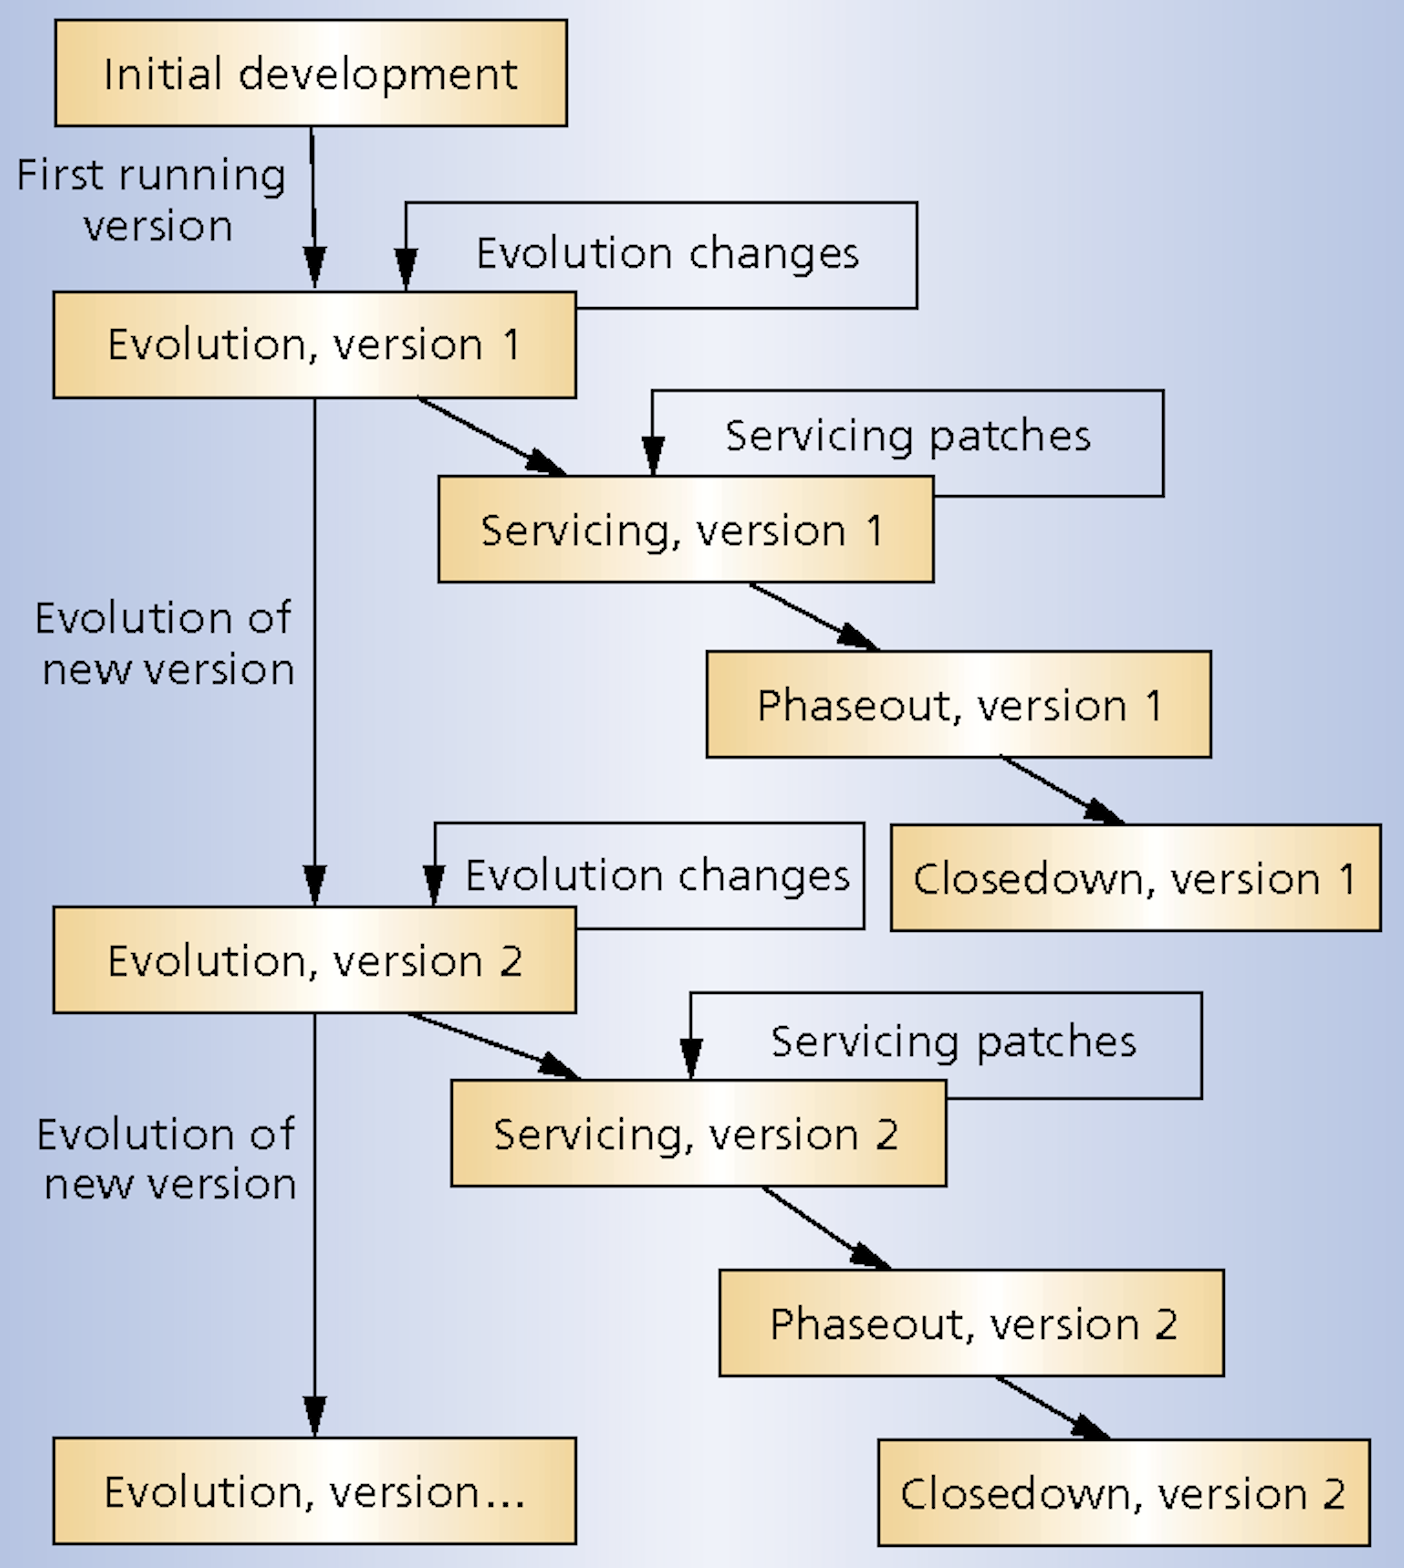
\includegraphics[scale=0.35]{JAI 2023/figures/staged-model-versions.png}
    \caption{\textit{O modelo de Rajlich com versões enfatiza a natureza evolutiva do desenvolvimento de software. Fonte:~\cite{rajlich:staged:2000}. }}
    \label{fig:staged:model}
\end{figure}

%Para o software de pesquisa, se existe um artigo de pesquisa que o utiliza, ...
%EXPLICAR que não há closedown... por causa da reprodutibilidade.
No contexto de desenvolvimento de \RS, 
deve-se considerar que ele se insere em um projeto de pesquisa que inclui \textit{dados e software}. 
No início do desenvolvimento do \RSw deve-se decidir
sobre a licença do software, onde o software será armazenado (por exemplo, GitHub, GitLab, etc.), tipo de sistema de versionamento e padrões de entrada e saída.
%
O lançamento de uma versão do \RSw e sua liberação para a sua comunidade podem ser motivados pela publicação de um artigo científico. O texto do artigo deve mencionar claramente a versão do \RSw utilizada. 

Também é essencial considerar a continuidade do \RSw ao longo do tempo e o suporte à  reprodutibilidade, especialmente quando o software for usado na pesquisa publicada em artigos científicos. 
Ao contrário de outros tipos de software, a etapa de Fechamento (\textit{Closedown}) não deveria ser considerada em \RSw para permitir a reprodutibilidade dos resultados divulgados nos artigos publicados.
Manter o \RSw vivo, disponível e acessível é fundamental para que outros cientistas possam reproduzir e verificar os resultados da pesquisa.

%\subsection{Dimensão Social}
\subsection{Pessoas} 

%A estrutura do grupo de pesquisa envolvido no desenvolvimento do software de pesquisa pode se refletir na estrutura do projeto ... 
%A pesquisa evolui, o grupo de pesquisa recebe novos membros, o software evolui, novo software pode ser criado que interfaceia com outros ...

%Holland: Many software maintenance problems are not technical but people problems\cite{versen_2020}
%We need to be able to organize the development team (group, community, etc.) in such a way that it embraces change and facilitates %maintenance and evolution, not only immediately after deployment of the software, but for the decades that follow.

Considerando que muitos problemas de manutenção de software não são problemas técnicos, mas problemas relacionados às pessoas~\cite{versen_2020}, percebemos que a dimensão social desempenha um papel importante na evolução do software, influenciando tanto o processo quanto o resultado final. 
As pessoas interessadas no desenvolvimento, utilização e manutenção de software têm um impacto significativo em sua evolução. A interação e colaboração entre os membros da equipe de desenvolvimento e os usuários contribuem com suas perspectivas e experiências, influenciando as decisões sobre novas funcionalidades, correções de \textit{bugs} e melhorias em geral. 
Além disso, as demandas e expectativas dos usuários, assim como  mudanças em suas necessidades e preferências podem exigir adaptações e atualizações do software para atender a essas demandas.

O caso específico da evolução de um \RSw  apresenta características distintas. 
O \RSw está inserido em um ecossistema científico, onde os pesquisadores buscam avançar o conhecimento em suas áreas. 
Nesse contexto, sua evolução está intimamente ligada à evolução da própria pesquisa e ao surgimento de novas abordagens e técnicas, exigindo atualizações e modificações no software. 
Além disso, a estrutura do grupo de pesquisa também influencia a evolução do software. À medida em que a pesquisa avança, novos membros ingressam no grupo, pesquisadores saem e a equipe se reconfigura. Tais mudanças na composição do grupo demandam mecanismos para transmitir o conhecimento legado e práticas estabelecidas.

%- Abrir para contribuição externa?
Tornar um \RSw disponível publicamente e aceitar contribuição de pessoas externas ao grupo de pesquisa pode resultar em uma comunidade maior de desenvolvedores envolvidos, facilitando o desenvolvimento mais rápido e eficiente, incluindo correções de \textit{bugs} e implementação de novos recursos de forma colaborativa. No entanto, a coordenação de um \RSw aberto pode exigir esforço adicional para estabelecer processos de governança e revisão de contribuições, para garantir que estas sejam de alta qualidade e estejam alinhadas com os objetivos do projeto. 
Além disso, a abertura precoce do \RSw pode expor pesquisas em andamento antes que estejam prontas para a publicação, o que pode comprometer a confidencialidade e ineditismo dos resultados.

%------------------------------------------
%\subsection{Práticas para o Desenvolvimento de Software} 

\subsection{Práticas} 

Há alguns anos a comunidade científica já reconhece ser essencial que cientistas, pesquisadores e estudantes sejam capazes de aprender e adotar um novo conjunto de habilidades e metodologias relacionadas a software~\cite{wssspe3}.
Alguns pesquisadores já abraçaram boas práticas de desenvolvimento de software e, em particular, uma classe especializada de desenvolvedores de software, chamados de \textit{Engenheiros de Software de Pesquisa} (\textit{Research Software Engineers}), está surgindo em ambientes acadêmicos como parte integrante de grupos de pesquisa bem-sucedidos~\cite{wssspe3}.
%
%\subsection{Ferramentas}
O uso consistente de boas práticas é apoiado por tecnologias e ferramentas conhecidas e tradicionalmente usadas por engenheiros de software.

%dentre elas, Git, Gitlab, Github, Docker.
%, bem como, ferramentas como R, Python, Latex, BibTex,  Workflow, Nextflow, etc etc.

\begin{comment}

\subsection{Engenheiros de Software de Pesquisa}

Engenheiros de Software de Pesquisa (\textit{Research Software Engineers}) ...
%
Engenharia de Software (engenheiro de software), Pesquisa (pesquisador).
%
O desenvolvimento de software de pesquisa requer indivíduos que combinem o melhor de ambas as funções (Figura~\ref{fig:rsengineering}).

\url{http://www.software.ac.uk/blog/2012-11-09-craftsperson-and-scholar}, \url{https://doi.org/10.5281/zenodo.7140726}. [KATZ]

\begin{figure}[htb]
    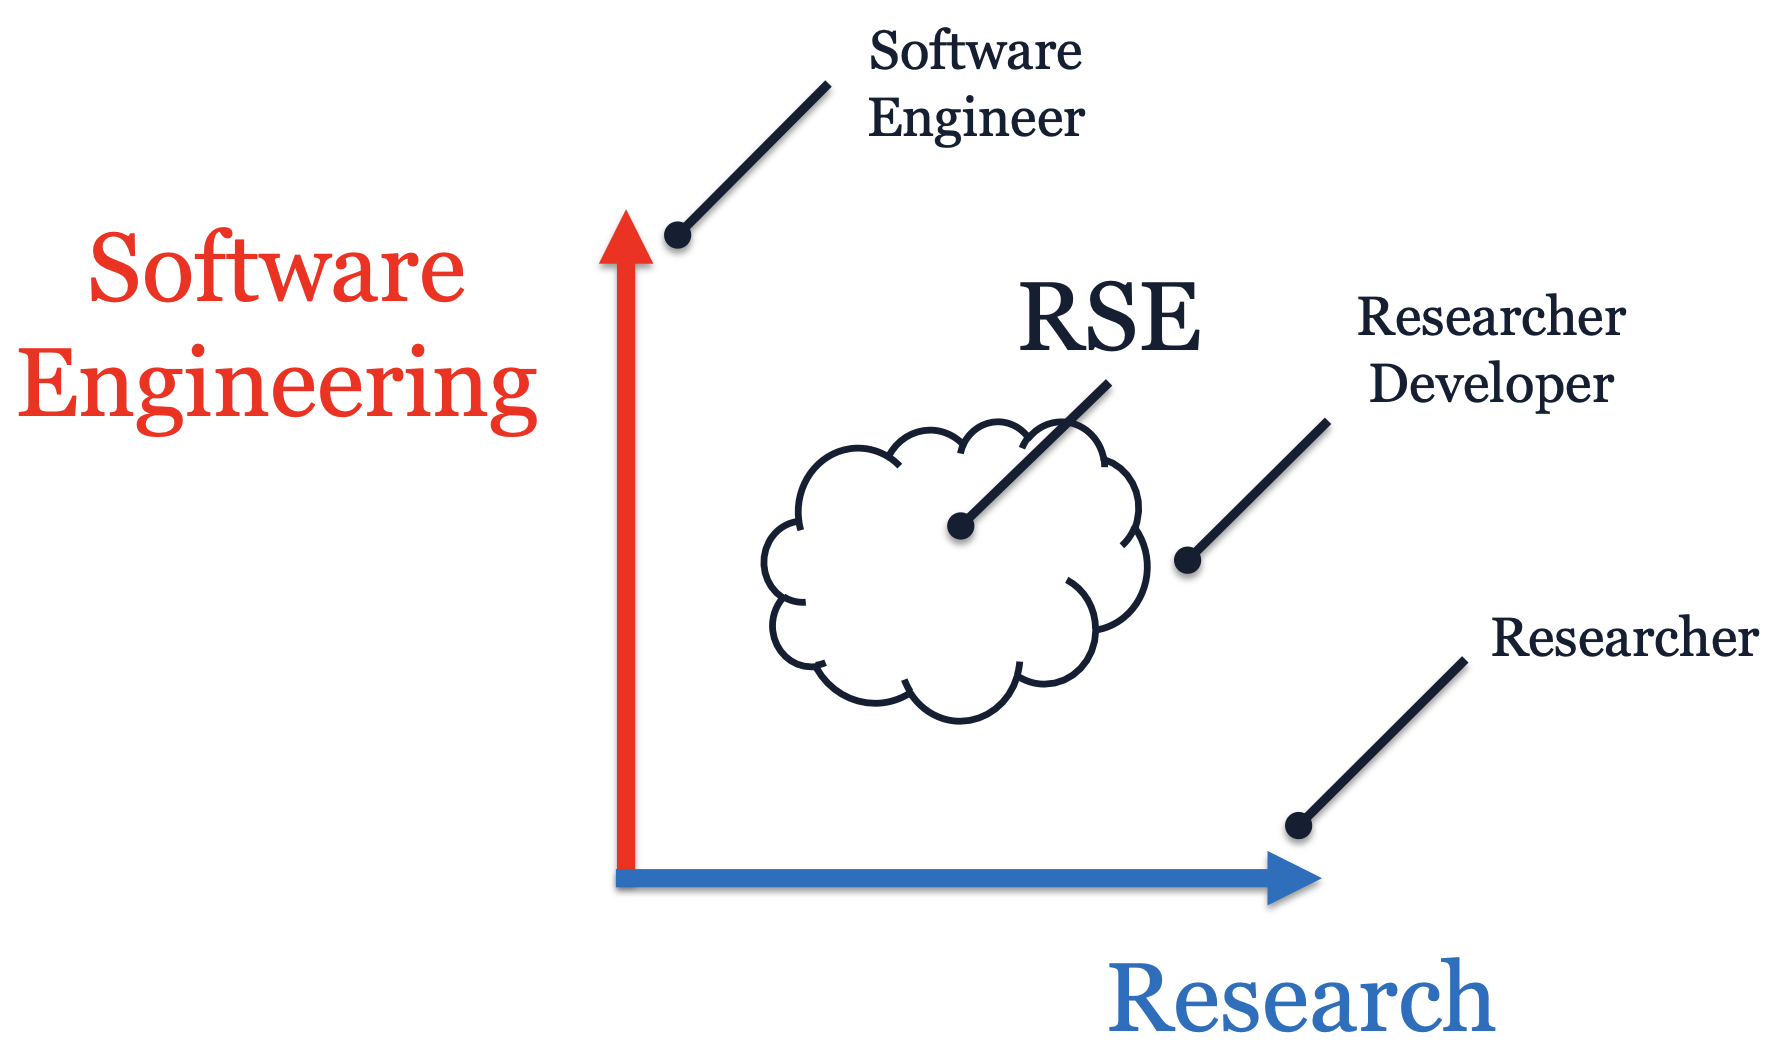
\includegraphics[scale=0.3]{JAI 2023/figures/research-software-engineering-katz.png}
    \caption{Caption [KATZ]}
    \label{fig:rsengineering}
\end{figure}

- Research Software Engineer (RSE)
+ Associations/societies
+ Career paths, structure

\end{comment}

% Alem da necessidade de politicas para melhorar a qualidade do codigo do software de pesquisa ha tambem a necessidade de politicas para incentivos a carreira do engenheiro de software de pesquisa e reconhecimento e visibilidade academica do seu trabalho.

%Desafios
%\begin{itemize}
%    \item Organizing and providing software training. 
     %Software-carpentry.org (http://software-carpentry.org/) provides the basic model to deliver that training.
%\end{itemize}


%--------------------------------%
%\subsection{Aspectos Avançados} %“I want to code better.” Provides more information on testing, continuous integration, release management, documentation, and other skills that help a programmer to produce higher-quality code.
%--------------------------------%
